\begin{center}
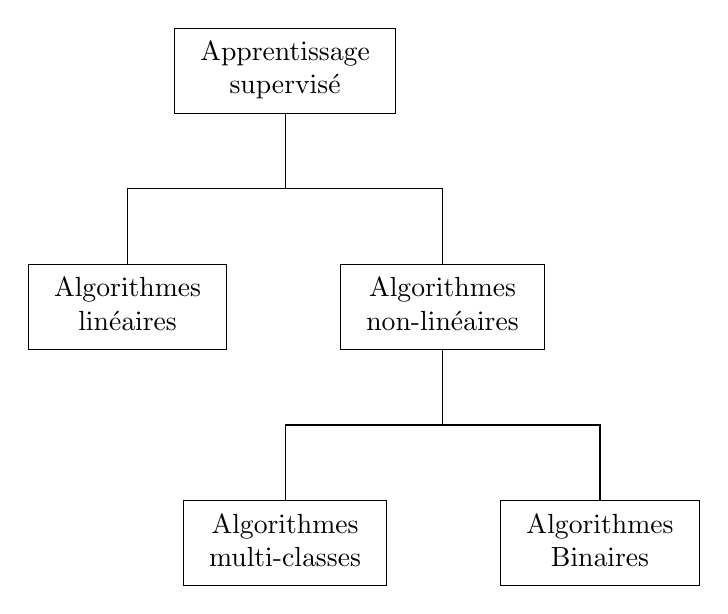
\begin{tikzpicture}
\begin{scope}
\node (AS) at (0,6) [rectangle,draw] {\begin{tabular}{c}Apprentissage\\ supervisé\end{tabular} };
\node (ASL) at (-2,3) [rectangle,draw] {\begin{tabular}{c}Algorithmes\\ linéaires\end{tabular} };
\node (ASNL) at (2,3) [rectangle,draw] {\begin{tabular}{c}Algorithmes\\ non-linéaires\end{tabular} };
\node (ASIM) at (0,0) [rectangle,draw] {\begin{tabular}{c}Algorithmes\\ multi-classes\end{tabular} };
\node (ASNM) at (4,0) [rectangle,draw] {\begin{tabular}{c}Algorithmes\\Binaires\end{tabular} };
\draw (AS) -- (0,4.5);
\draw (0,4.5) -| (ASNL);
\draw (0,4.5) -| (ASL);
\draw (ASNL) -- (2,1.5);
\draw (2,1.5) -| (ASIM);
\draw (2,1.5) -| (ASNM);
\end{scope}
\end{tikzpicture}
\end{center}
